\documentclass[10pt]{beamer}

\usetheme{metropolis}
\usepackage{appendixnumberbeamer}

\usepackage{booktabs,empheq,bbold,bm}
\usepackage[scale=2]{ccicons}

\usepackage{pgfplots}
\usepgfplotslibrary{dateplot}

\usepackage{xspace}
\newcommand{\themename}{\textbf{\textsc{metropolis}}\xspace}

\newcommand{\bn}{\mathbf{n}}
\newcommand{\bq}{\mathbf{q}}
\newcommand{\bu}{\mathbf{u}}

\newcommand{\hbn}{\hat{\mathbf{n}}}
\newcommand{\hbx}{\hat{\mathbf{x}}}
\newcommand{\hbz}{\hat{\mathbf{z}}}

\newcommand{\bU}{\mathbf{U}}

\newcommand{\bpsi}{\bm{\psi}}
\newcommand{\bzero}{\bm{0}}

\newcommand{\eps}{\epsilon}
\newcommand{\grad}{\nabla}
\newcommand{\Div}{\nabla\cdot}

\newcommand{\rhoi}{\rho_{\text{i}}}

\newcommand{\comm}[1]{{\footnotesize \hfill \emph{#1}}}

\title{numerical modeling of glaciers}
%\subtitle{A modern beamer theme}
\date{June 2024}
\author{Ed Bueler}
\institute{the Hardware Store at McCarthy}
\titlegraphic{\vspace{-1cm}\par\hspace{-1cm}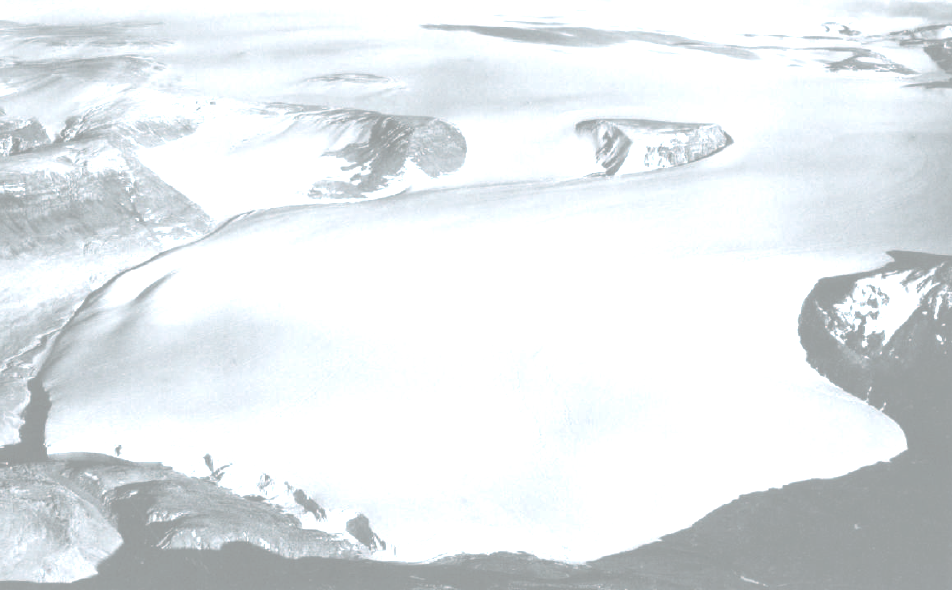
\includegraphics[width=1.5\textwidth]{polaris-overexposed.png}}

\begin{document}
\graphicspath{{../figures/}}

\maketitle

\begin{frame}{Outline}
  %\setbeamertemplate{section in toc}[sections numbered]
  %\tableofcontents[hideallsubsections]
  \tableofcontents
\end{frame}

\section{\textbf{hour 1: what happens at the surface of a glacier?}}

\subsection{basics}

\begin{frame}{surface motion}
  \begin{center}
  FIXME boat/slider pic full screen
  \end{center}
\end{frame}

\begin{frame}{surface motion: notation}
  \begin{center}
  FIXME boat/slider pic 1/3 screen
  \end{center}

\begin{itemize}
\item two spatial dimensions $x,z$ \hfill \emph{\dots\, at least for a while}
\item $z = s(t,x)$: ice surface elevation (m)
\item $z = b(x)$: (fixed) bed elevation (m)
\item $a(t,x)$: surface mass balance in ice-equivalent units ($\text{m}\,\text{s}^{-1}$)
\item $\bu(t,x)=(u(t,x),w(t,x))$: ice velocity ($\text{m}\,\text{s}^{-1}$)
\end{itemize}
\end{frame}

\begin{frame}{surface kinematical equation (SKE)}
  \begin{center}
  FIXME boat/slider pic 1/3 screen
  \end{center}

\begin{equation*}
\frac{\partial s}{\partial t} = \uncover<2-4>{a} \uncover<3-4>{+w} \uncover<4>{-u \frac{\partial s}{\partial x}}
\end{equation*}

the surface moves up and down according to
\begin{itemize}
\item<2-4> surface mass balance
\item<3-4> vertical ice velocity
\item<4> horizontal ice velocity
\end{itemize}
\end{frame}

\begin{frame}{surface kinematical equation (SKE) \dots alternate form}
  \begin{center}
  FIXME boat/slider pic 1/3 screen
  \end{center}

\begin{equation*}
\frac{\partial s}{\partial t} = a + \bu \cdot \bn_s
\end{equation*}

\begin{itemize}
\item $\bu=(u,w)$ is the ice velocity
\item $\bn_s$ is a vector which points upward and is normal (perpendicular) to the ice surface:
	$$\bn_s = \left(-\frac{\partial s}{\partial x}, \,1\right)$$
\end{itemize}
\end{frame}

\subsection{numerics}

\begin{frame}[fragile]{Typography}
      \begin{verbatim}The theme provides sensible defaults to
\emph{emphasize} text, \alert{accent} parts
or show \textbf{bold} results.\end{verbatim}

  \begin{center}becomes\end{center}

  The theme provides sensible defaults to \emph{emphasize} text,
  \alert{accent} parts or show \textbf{bold} results.
\end{frame}

\begin{frame}{Font feature test}
  \begin{itemize}
    \item Regular
    \item \textit{Italic}
    \item \textsc{Small Caps}
    \item \textbf{Bold}
    \item \textbf{\textit{Bold Italic}}
    \item \textbf{\textsc{Bold Small Caps}}
    \item \texttt{Monospace}
    \item \texttt{\textit{Monospace Italic}}
    \item \texttt{\textbf{Monospace Bold}}
    \item \texttt{\textbf{\textit{Monospace Bold Italic}}}
  \end{itemize}
\end{frame}

\begin{frame}{Lists}
  \begin{columns}[T,onlytextwidth]
    \column{0.33\textwidth}
      Items
      \begin{itemize}
        \item Milk \item Eggs \item Potatoes
      \end{itemize}

    \column{0.33\textwidth}
      Enumerations
      \begin{enumerate}
        \item First, \item Second and \item Last.
      \end{enumerate}

    \column{0.33\textwidth}
      Descriptions
      \begin{description}
        \item[PowerPoint] Meeh. \item[Beamer] Yeeeha.
      \end{description}
  \end{columns}
\end{frame}


\begin{frame}{Figures}
  \begin{figure}
    \newcounter{density}
    \setcounter{density}{20}
    \begin{tikzpicture}
      \def\couleur{alerted text.fg}
      \path[coordinate] (0,0)  coordinate(A)
                  ++( 90:5cm) coordinate(B)
                  ++(0:5cm) coordinate(C)
                  ++(-90:5cm) coordinate(D);
      \draw[fill=\couleur!\thedensity] (A) -- (B) -- (C) --(D) -- cycle;
      \foreach \x in {1,...,40}{%
          \pgfmathsetcounter{density}{\thedensity+20}
          \setcounter{density}{\thedensity}
          \path[coordinate] coordinate(X) at (A){};
          \path[coordinate] (A) -- (B) coordinate[pos=.10](A)
                              -- (C) coordinate[pos=.10](B)
                              -- (D) coordinate[pos=.10](C)
                              -- (X) coordinate[pos=.10](D);
          \draw[fill=\couleur!\thedensity] (A)--(B)--(C)-- (D) -- cycle;
      }
    \end{tikzpicture}
    \caption{Rotated square from
    \href{http://www.texample.net/tikz/examples/rotated-polygons/}{texample.net}.}
  \end{figure}
\end{frame}

\begin{frame}{Blocks}
  Three different block environments are pre-defined and may be styled with an
  optional background color.

  \begin{columns}[T,onlytextwidth]
    \column{0.5\textwidth}
      \begin{block}{Default}
        Block content.
      \end{block}

      \begin{alertblock}{Alert}
        Block content.
      \end{alertblock}

      \begin{exampleblock}{Example}
        Block content.
      \end{exampleblock}

    \column{0.5\textwidth}

      \metroset{block=fill}

      \begin{block}{Default}
        Block content.
      \end{block}

      \begin{alertblock}{Alert}
        Block content.
      \end{alertblock}

      \begin{exampleblock}{Example}
        Block content.
      \end{exampleblock}

  \end{columns}
\end{frame}

\begin{frame}{Line plots}
  \begin{figure}
    \begin{tikzpicture}
      \begin{axis}[
        mlineplot,
        width=0.9\textwidth,
        height=6cm,
      ]

        \addplot {sin(deg(x))};
        \addplot+[samples=100] {sin(deg(2*x))};

      \end{axis}
    \end{tikzpicture}
  \end{figure}
\end{frame}

\begin{frame}{Quotes}
  \begin{quote}
    Veni, Vidi, Vici
  \end{quote}
\cite{knuth92,ConcreteMath,Simpson,Er01,greenwade93}
\end{frame}

{%
\setbeamertemplate{frame footer}{My custom footer}
\begin{frame}[fragile]{Frame footer}
    \themename defines a custom beamer template to add a text to the footer. It can be set via
    \begin{verbatim}\setbeamertemplate{frame footer}{My custom footer}\end{verbatim}
\end{frame}
}


\section{\textbf{hour 2: where does the velocity field come from?}}

\subsection{basics}


\begin{frame}{ice in glaciers is an atypical fluid}

\begin{itemize}
\item if the ice were
  \begin{itemize}
  \item[$\circ$] faster-moving than it actually is, and
  \item[$\circ$] linearly-viscous like liquid water
  \end{itemize}

  then it would be a ``typical'' fluid

\bigskip
\item for typical fluids one uses the Navier-Stokes equations:
\begin{align*}
\nabla \cdot \mathbf{u} &= 0 &&\text{\emph{incompressibility}} \\
\rho \left(\mathbf{u}_t + \mathbf{u}\cdot\nabla \mathbf{u}\right) &= -\nabla p + \nabla \cdot \tau_{ij} + \rho \mathbf{g} &&\text{\emph{stress balance}} \\
2 \nu D\mathbf{u}_{ij} &= \tau_{ij} &&\text{\emph{flow law}}
\end{align*}

\medskip
    \begin{itemize}
    \item[$\circ$] stress balance equation is ``$m a = F$''
    \end{itemize}
\end{itemize}
\end{frame}


\begin{frame}{glaciology as computational fluid dynamics}

\begin{itemize}
\item \alert{yes}, numerical ice sheet flow modelling is ``computational fluid dynamics''
  \begin{itemize}
  \item[$\circ$] it's large-scale like atmosphere and ocean
  \item[$\circ$] \dots\, but it is a weird one
  \end{itemize}
\item consider what makes atmosphere/ocean flow exciting:
  \begin{itemize}
  \item[$\circ$] turbulence
  \item[$\circ$] convection
  \item[$\circ$] coriolis force
  \item[$\circ$] density stratification
  \end{itemize}
\item none of the above list is relevant to ice flow
\item what could be interesting about the flow of slow, cold, stiff, laminar, inert old ice?
  \begin{itemize}
  \item[$\circ$] \emph{ice dynamics!}
  \end{itemize}
\end{itemize}
\end{frame}


\begin{frame}{ice is a slow, shear-thinning fluid}

\begin{itemize}
\item ice fluid is \emph{slow} and \emph{non-Newtonian}
    \begin{itemize}
    \item[$\circ$] ``slow'' is a technical term:
      $$\rho \left(\mathbf{u}_t + \mathbf{u}\cdot\nabla \mathbf{u}\right) \approx 0 \qquad \iff \qquad \begin{pmatrix} \text{forces of inertia} \\ \text{are neglected} \end{pmatrix}$$
    \item[$\circ$] ice is non-Newtonian in a ``shear-thinning'' way
        \begin{itemize}
        \item higher strain rates means lower viscosity
        \item viscosity $\nu$ is not constant
        \end{itemize}
    \end{itemize}

\bigskip
\item thus the standard model is Glen-law Stokes:
\begin{align*}
\nabla \cdot \mathbf{u} &= 0 &&\text{\emph{incompressibility}} \\
0 &= - \nabla p + \nabla \cdot \tau_{ij} + \rho\, \mathbf{g} &&\text{\emph{stress balance}} \\
D\mathbf{u}_{ij} &= A \tau^{n-1} \tau_{ij} &&\text{\emph{flow law}}
\end{align*}

\end{itemize}
\end{frame}


\begin{frame}{``slow'' means no memory of velocity/momentum}

\begin{itemize}
\item note \emph{no time derivatives} in Stokes model:
\small
\begin{align*}
\nabla \cdot \mathbf{u} &= 0 \\
0 &= - \nabla p + \nabla \cdot \tau_{ij} + \rho\, \mathbf{g} \\
D\mathbf{u}_{ij} &= A \tau^{n-1} \tau_{ij}
\end{align*}
\normalsize
\item thus a time-stepping ice sheet code can/must recompute the full velocity field at every time step
  \begin{itemize}
  \item[$\circ$] velocity is \emph{not} required from the previous time step
  \item[$\circ$] velocity is a ``diagnostic'' output not needed for starting or restarting the model
  \end{itemize}
\end{itemize}
\end{frame}


\begin{frame}{plane flow Stokes}

\begin{itemize}
\item again we work in a $x,z$ plane
    \begin{itemize}
    \item[$\circ$] glacier flow line (center line), or a cross-flow plane
    \end{itemize}
\item $n=3$ Stokes equations say:
\begin{empheq}[]{align}
u_x + w_z &= 0 &&\text{\emph{incompressibility}}\notag \\
p_x &= \tau_{11,x} + \tau_{13,z} &&\text{\emph{stress balance} ($x$)} \notag \\
p_z &= \tau_{13,x} - \tau_{11,z} - \rho g &&\text{\emph{stress balance} ($z$)} \notag \\
u_x &= A \tau^2 \tau_{11} &&\text{\emph{flow law (diagonal)}}\notag \\
u_z + w _x &= 2 A \tau^2 \tau_{13} &&\text{\emph{flow law (off-diagonal)}} \notag
\end{empheq}

\vspace{-2mm}
    \begin{itemize}
    \item[$\circ$] \emph{notation}: subscripts $x,z$ denote partial derivatives, $\tau_{13}$ is the ``vertical'' shear stress, $\tau_{11}$ and $\tau_{33}=-\tau_{11}$ are (deviatoric) longitudinal stresses
    \end{itemize}
\item we have five equations in five unknowns ($u,w,p,\tau_{11},\tau_{13}$)
\item this is complicated enough \dots what about in a simplified situation?
\end{itemize}
\end{frame}


\begin{frame}{slab-on-a-slope}

\hfill \includegraphics[width=0.4\textwidth]{slab}

\vspace{-30mm}
\begin{itemize}
\item suppose constant thickness
\item tilt bedrock by angle $\alpha$
\item rotate the coordinates
\item get replacement expressions:
\begin{align*}
\mathbf{g} &= g \sin\alpha\, \hat x - g \cos \alpha \,\hat z \phantom{dslfkj sdkfjlskdjf  sdlfj}\\
p_x &= \tau_{11,x} + \tau_{13,z} + \rho g \sin\alpha \\
p_z &= \tau_{13,x} - \tau_{11,z} - \rho g \cos\alpha
\end{align*}
\item for \alert{slab-on-a-slope} there is \emph{no variation in} $x$:\quad $\partial/\partial x = 0$
\item the equations simplify:
\small
\begin{empheq}[box=\fbox]{align}
w_z &= 0 &   0 &= \tau_{11} \notag \\
\tau_{13,z} &= - \rho g \sin\alpha &   u_z &= 2 A \tau^2 \tau_{13} \notag \\
p_z &= - \rho g \cos\alpha \notag
\end{empheq}
\end{itemize}
\end{frame}


\begin{frame}{slab-on-a-slope 2}

\begin{itemize}
\item add boundary conditions:
	$$w(\text{base})=0, \qquad p(\text{surface})=0, \qquad u(\text{base})=u_0$$
\item by integrating vertically, get:
\begin{align*}
w &= 0 \phantom{asdfklj asldkfjalk asdfkj sdlfkj sldafkj adlfjl sdfakj }\\
p &= \rho g \cos\alpha (H-z) \\
\tau_{13} &= \rho g \sin\alpha (H-z)
\end{align*}

\vspace{-25mm}
\hfill \includegraphics[width=0.4\textwidth]{slabshear}

\vspace{-7mm}
\item $\tau_{13}$ is linear in depth

\medskip
\item from $u_z = 2 A \tau^2 \tau_{13}$ get \alert{velocity formula}
\vspace{-0.05in}
\begin{align*}
u(z) &= u_0 + 2 A (\rho g \sin\alpha)^3 \int_0^z (H-z')^3\,dz' \\
     &= u_0 + \frac{1}{2} A (\rho g \sin\alpha)^3  \left(H^4 - (H-z)^4\right)
\end{align*}
\end{itemize}
\end{frame}


\begin{frame}{slab-on-a-slope 3}

\begin{columns}
\begin{column}{0.6\textwidth}
\begin{itemize}
\item do we believe these equations?
\item velocity formula on last slide gives figure below
\item compare to observations at right
\end{itemize}
\begin{center}
% NOT preserving aspect ratio
\includegraphics[width=0.6\textwidth,height=0.5\textheight]{slabvel}
\end{center}
\end{column}

\begin{column}{0.4\textwidth}
\includegraphics[width=1.0\textwidth]{athabasca-deform}

\medskip
\scriptsize
Velocity profile of the Athabasca Glacier, Canada, derived from inclinometry (Savage and Paterson, 1963)
\end{column}
\end{columns}
\end{frame}


\subsection{numerics}

\begin{frame}{Summary}
FIXME
\end{frame}

\begin{frame}[standout]
  Questions?
\end{frame}

\appendix

\begin{frame}[allowframebreaks]{References}
  \bibliography{slides}
  \bibliographystyle{abbrv}
\end{frame}


\subsection[]{extra slides}

\begin{frame}{extra: SKE from mass conservation}
\begin{center}
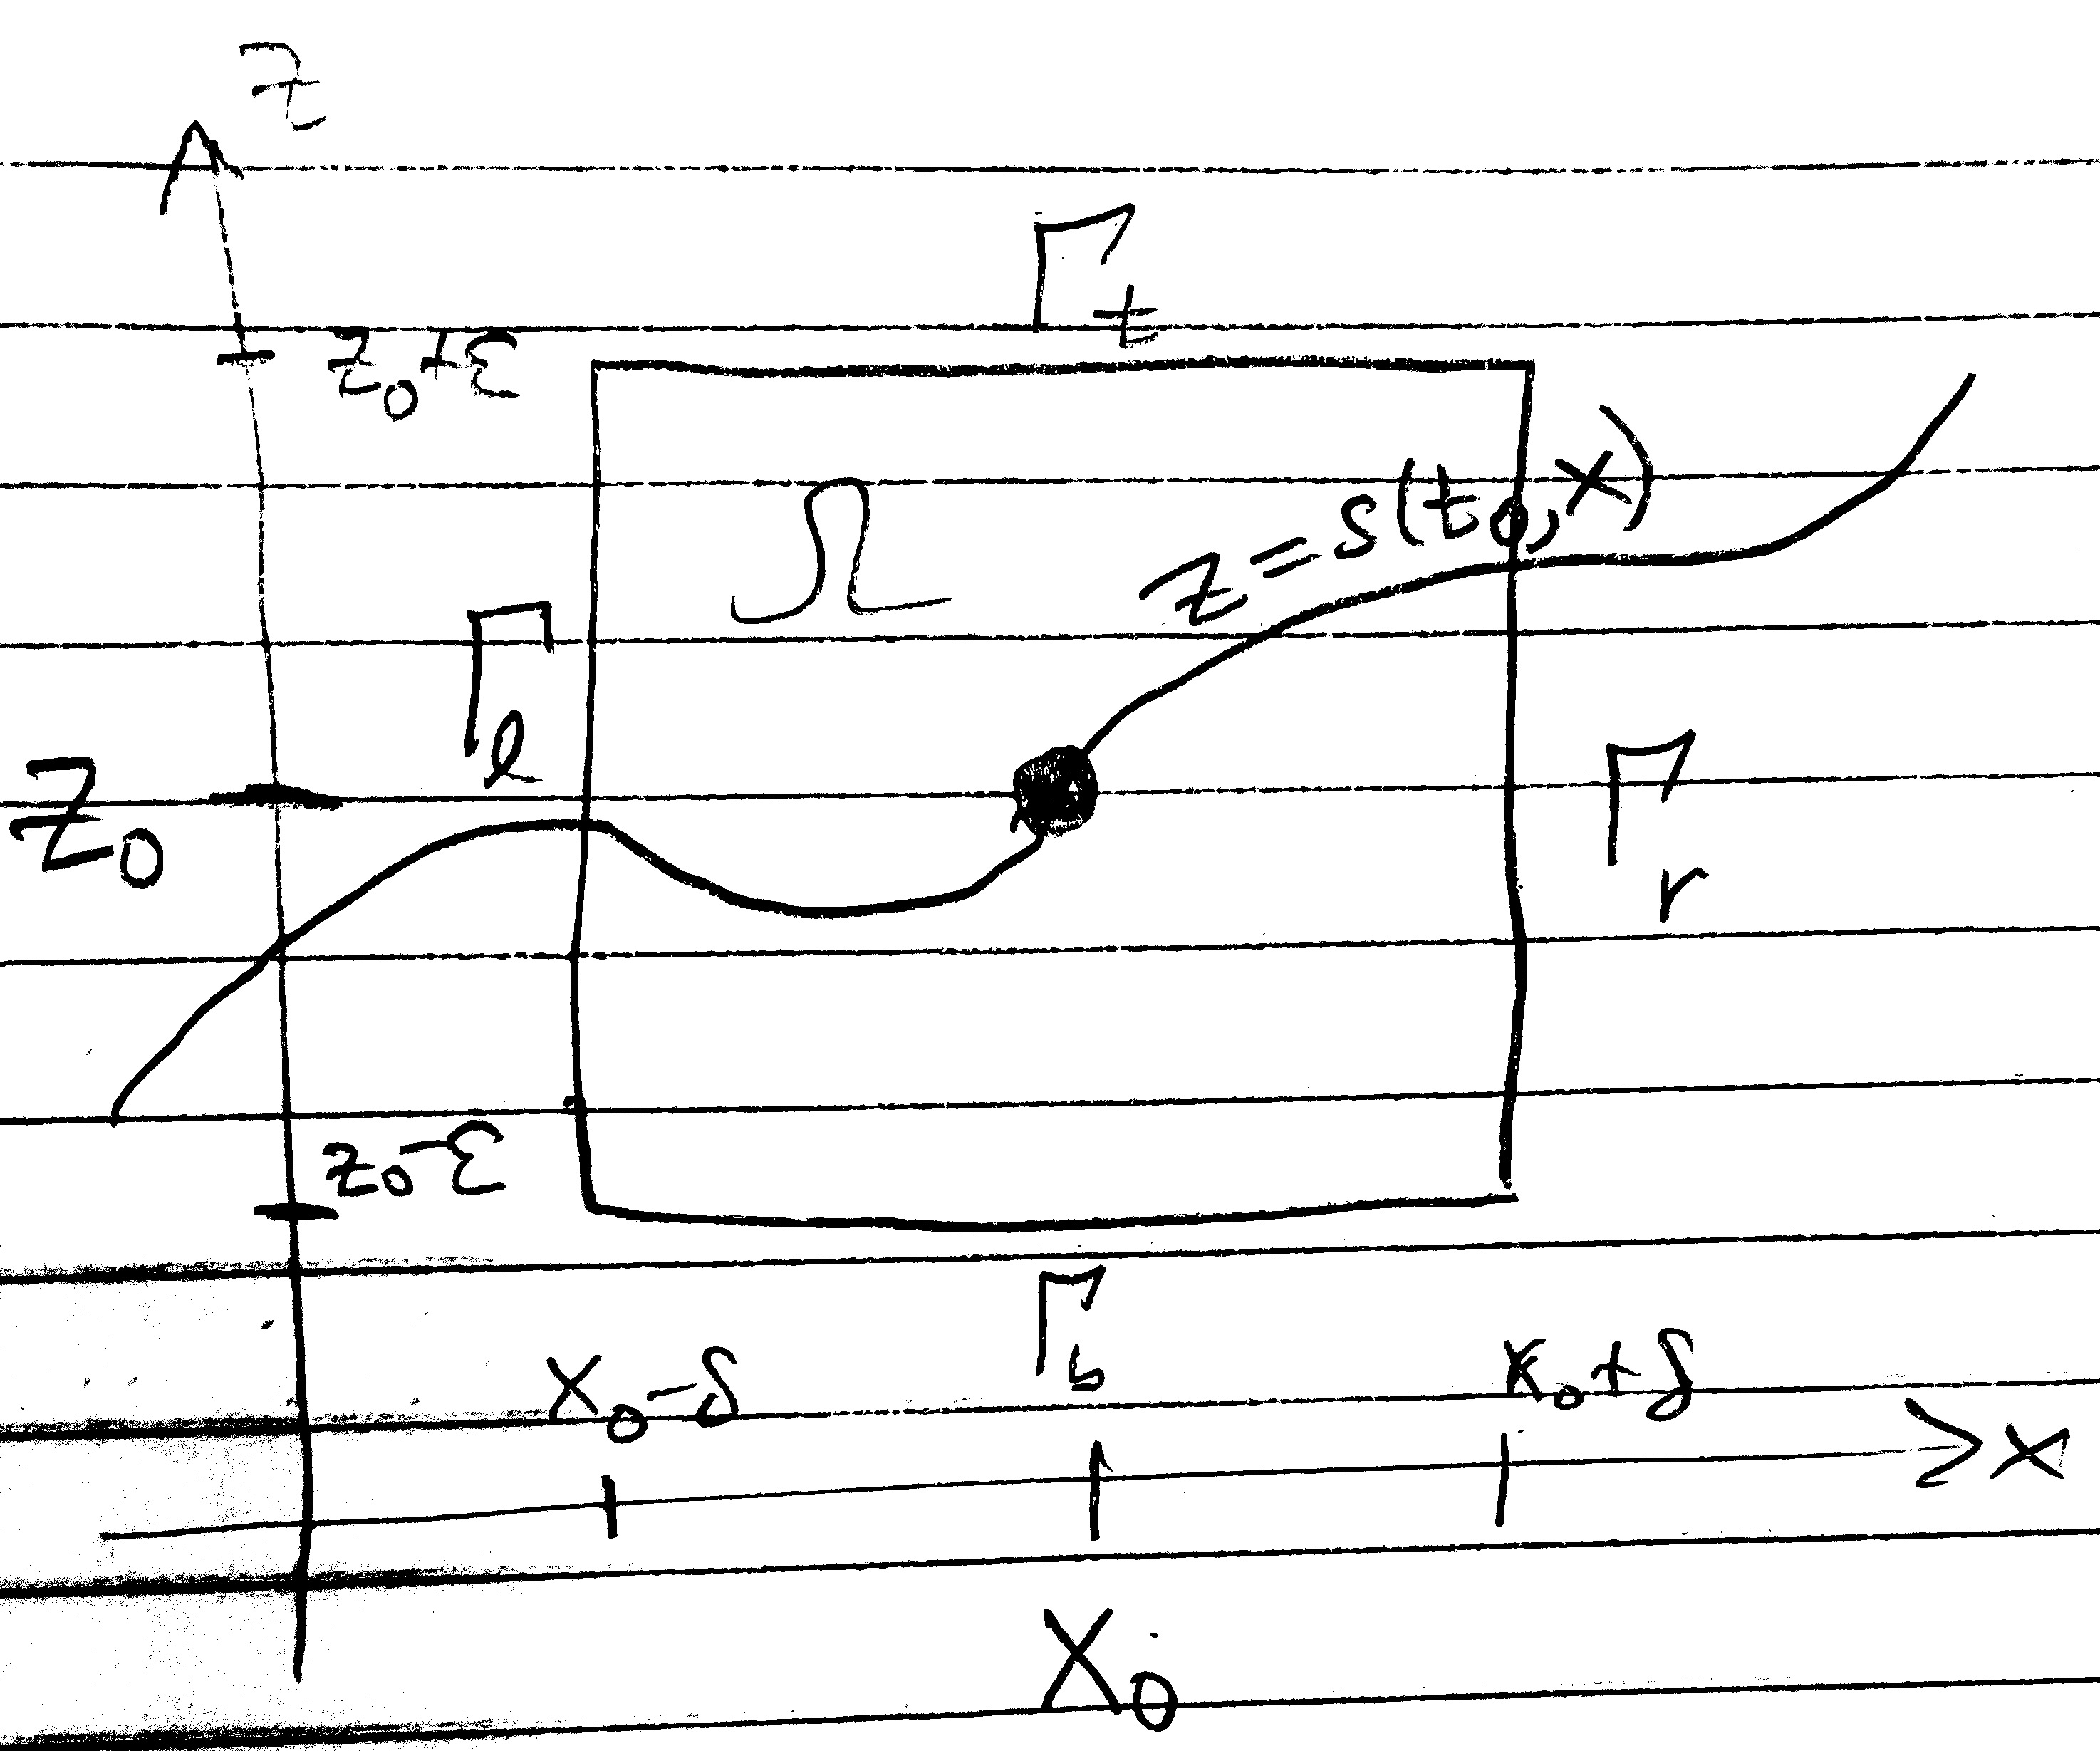
\includegraphics[width=0.3\textwidth]{skemassconservation.jpg}
\end{center}

\begin{itemize}
\item derive SKE from mass conservation over rectangle centered at $(x_0,z_0)$, where $s(t_0,x_0)=z_0$:
   $$\Omega=[x_0-\delta,x_0+\delta] \times [z_0-\eps,z_0+\eps]$$
\item define mass of ice in $\Omega$ at time $t$ as $M(t)$:
   $$M(t) = \rhoi \int_\Omega \mathbb{1}_{\{z<s(t,x)\}}\,dx\,dz = \rhoi \int_{x_0-\delta}^{x_0+\delta} s(t,x) - z_0 + \eps\,dx$$
\item also define:
   \begin{itemize}
   \item[$\circ$] $\bpsi$ is the mass flux
   \item[$\circ$] $\hbn$ is unit outward normal on $\partial\Omega$
   \end{itemize}
\end{itemize}
\end{frame}

\begin{frame}{extra: SKE from mass conservation 2}
\begin{center}
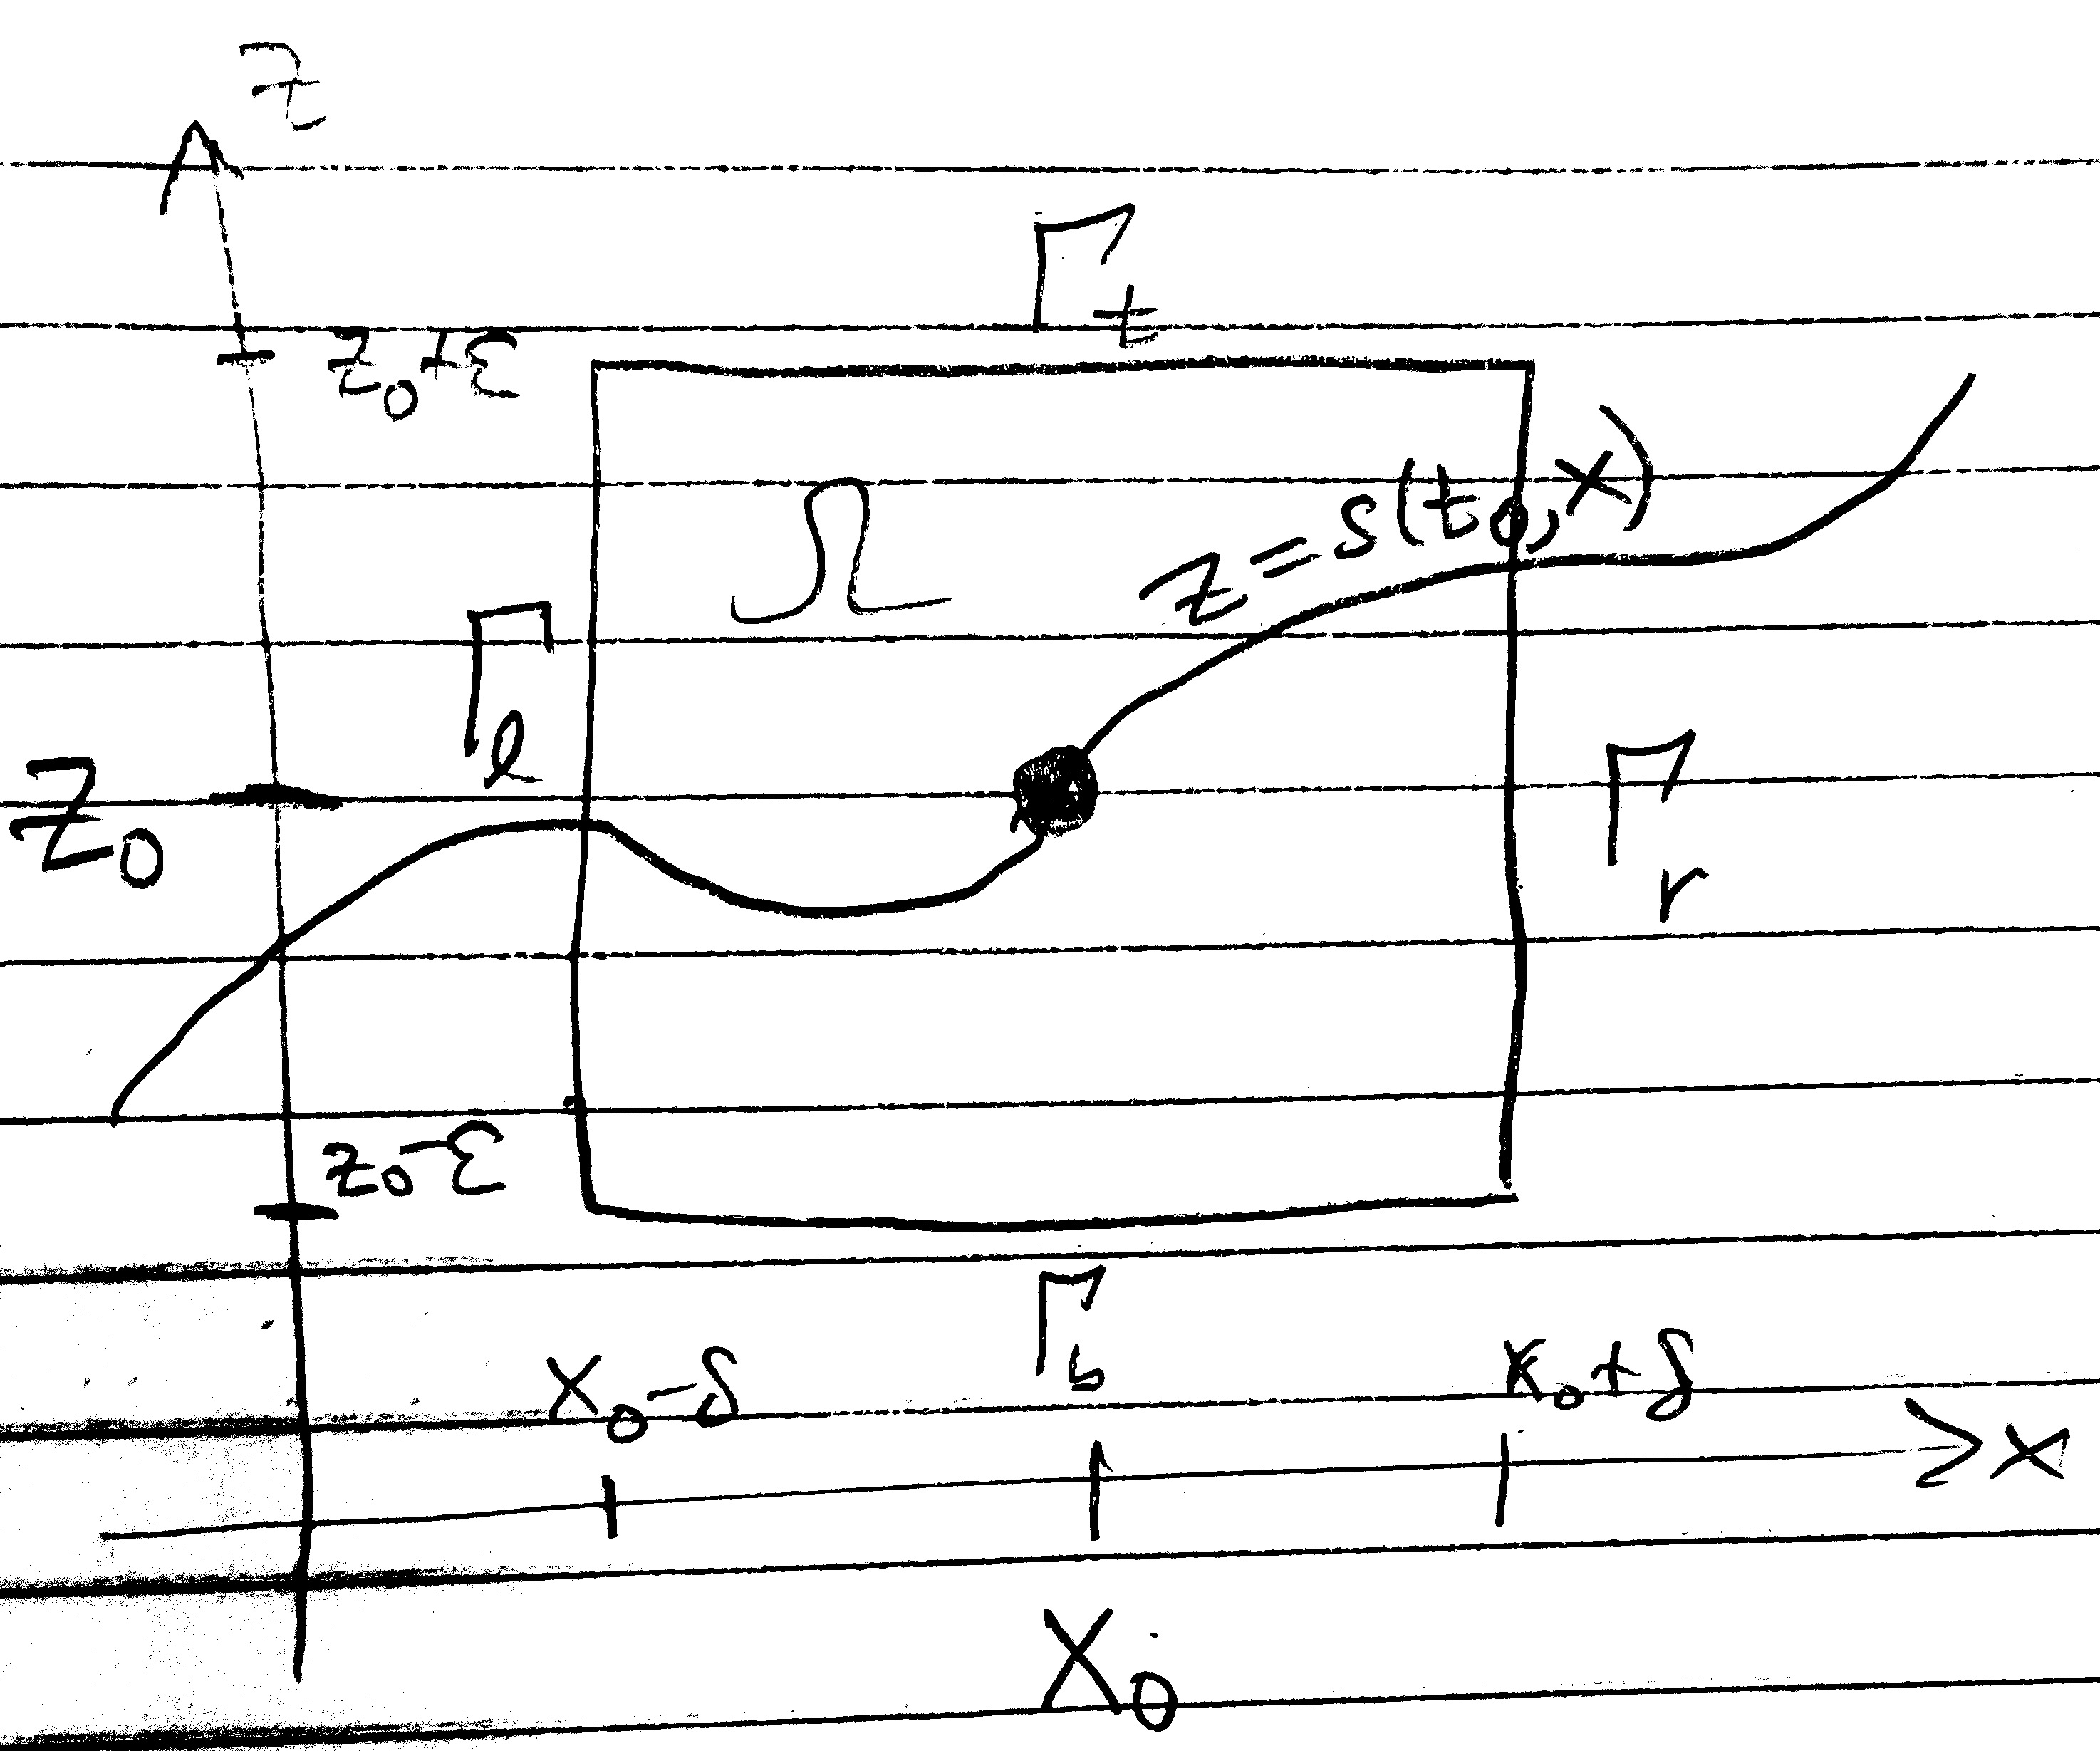
\includegraphics[width=0.3\textwidth]{skemassconservation.jpg}
\end{center}

\begin{itemize}
\item assumptions:
    \begin{itemize}
    \item[$\circ$] there is $\tau>0$ so that, for each $t$ such that $|t-t_0|<\tau$ the functions $s(t,x)$ are well-defined and $|s(t,x)-z_0|<\eps$
    \item[$\circ$] ice has constant density $\rhoi$
    \item[$\circ$] the SMB $a(t,x)$ only crosses the top boundary $\Gamma_t$ \hfill \emph{tentative}
        \begin{itemize}
        \item $\bpsi\big|_{\Gamma_t} = - \rho_i a(t,x) \hbz$  \comm{note $a>0$ is precipitation}
        \end{itemize}
    \item[$\circ$] $\bu(t,x,z)=(u,w)$ is the ice velocity  \comm{only defined on $\{z<s(t,x)\}$}
        \begin{itemize}
        \item $\bpsi\big|_{\Gamma_b} = \rho_i w(t,x,z_0-\eps) \hbz$
        \item $\bpsi\big|_{\Gamma_{\{\ell,r\}}} = \begin{cases} \rho_i u(t,x_0\mp\delta,z) \hbx, & \text{if } z < s(t,x_0\mp\delta), \\ \bzero, & \text{otherwise} \end{cases}$
        \end{itemize}
    \end{itemize}
\end{itemize}
\end{frame}

\begin{frame}{extra: SKE from mass conservation 3}
\begin{center}
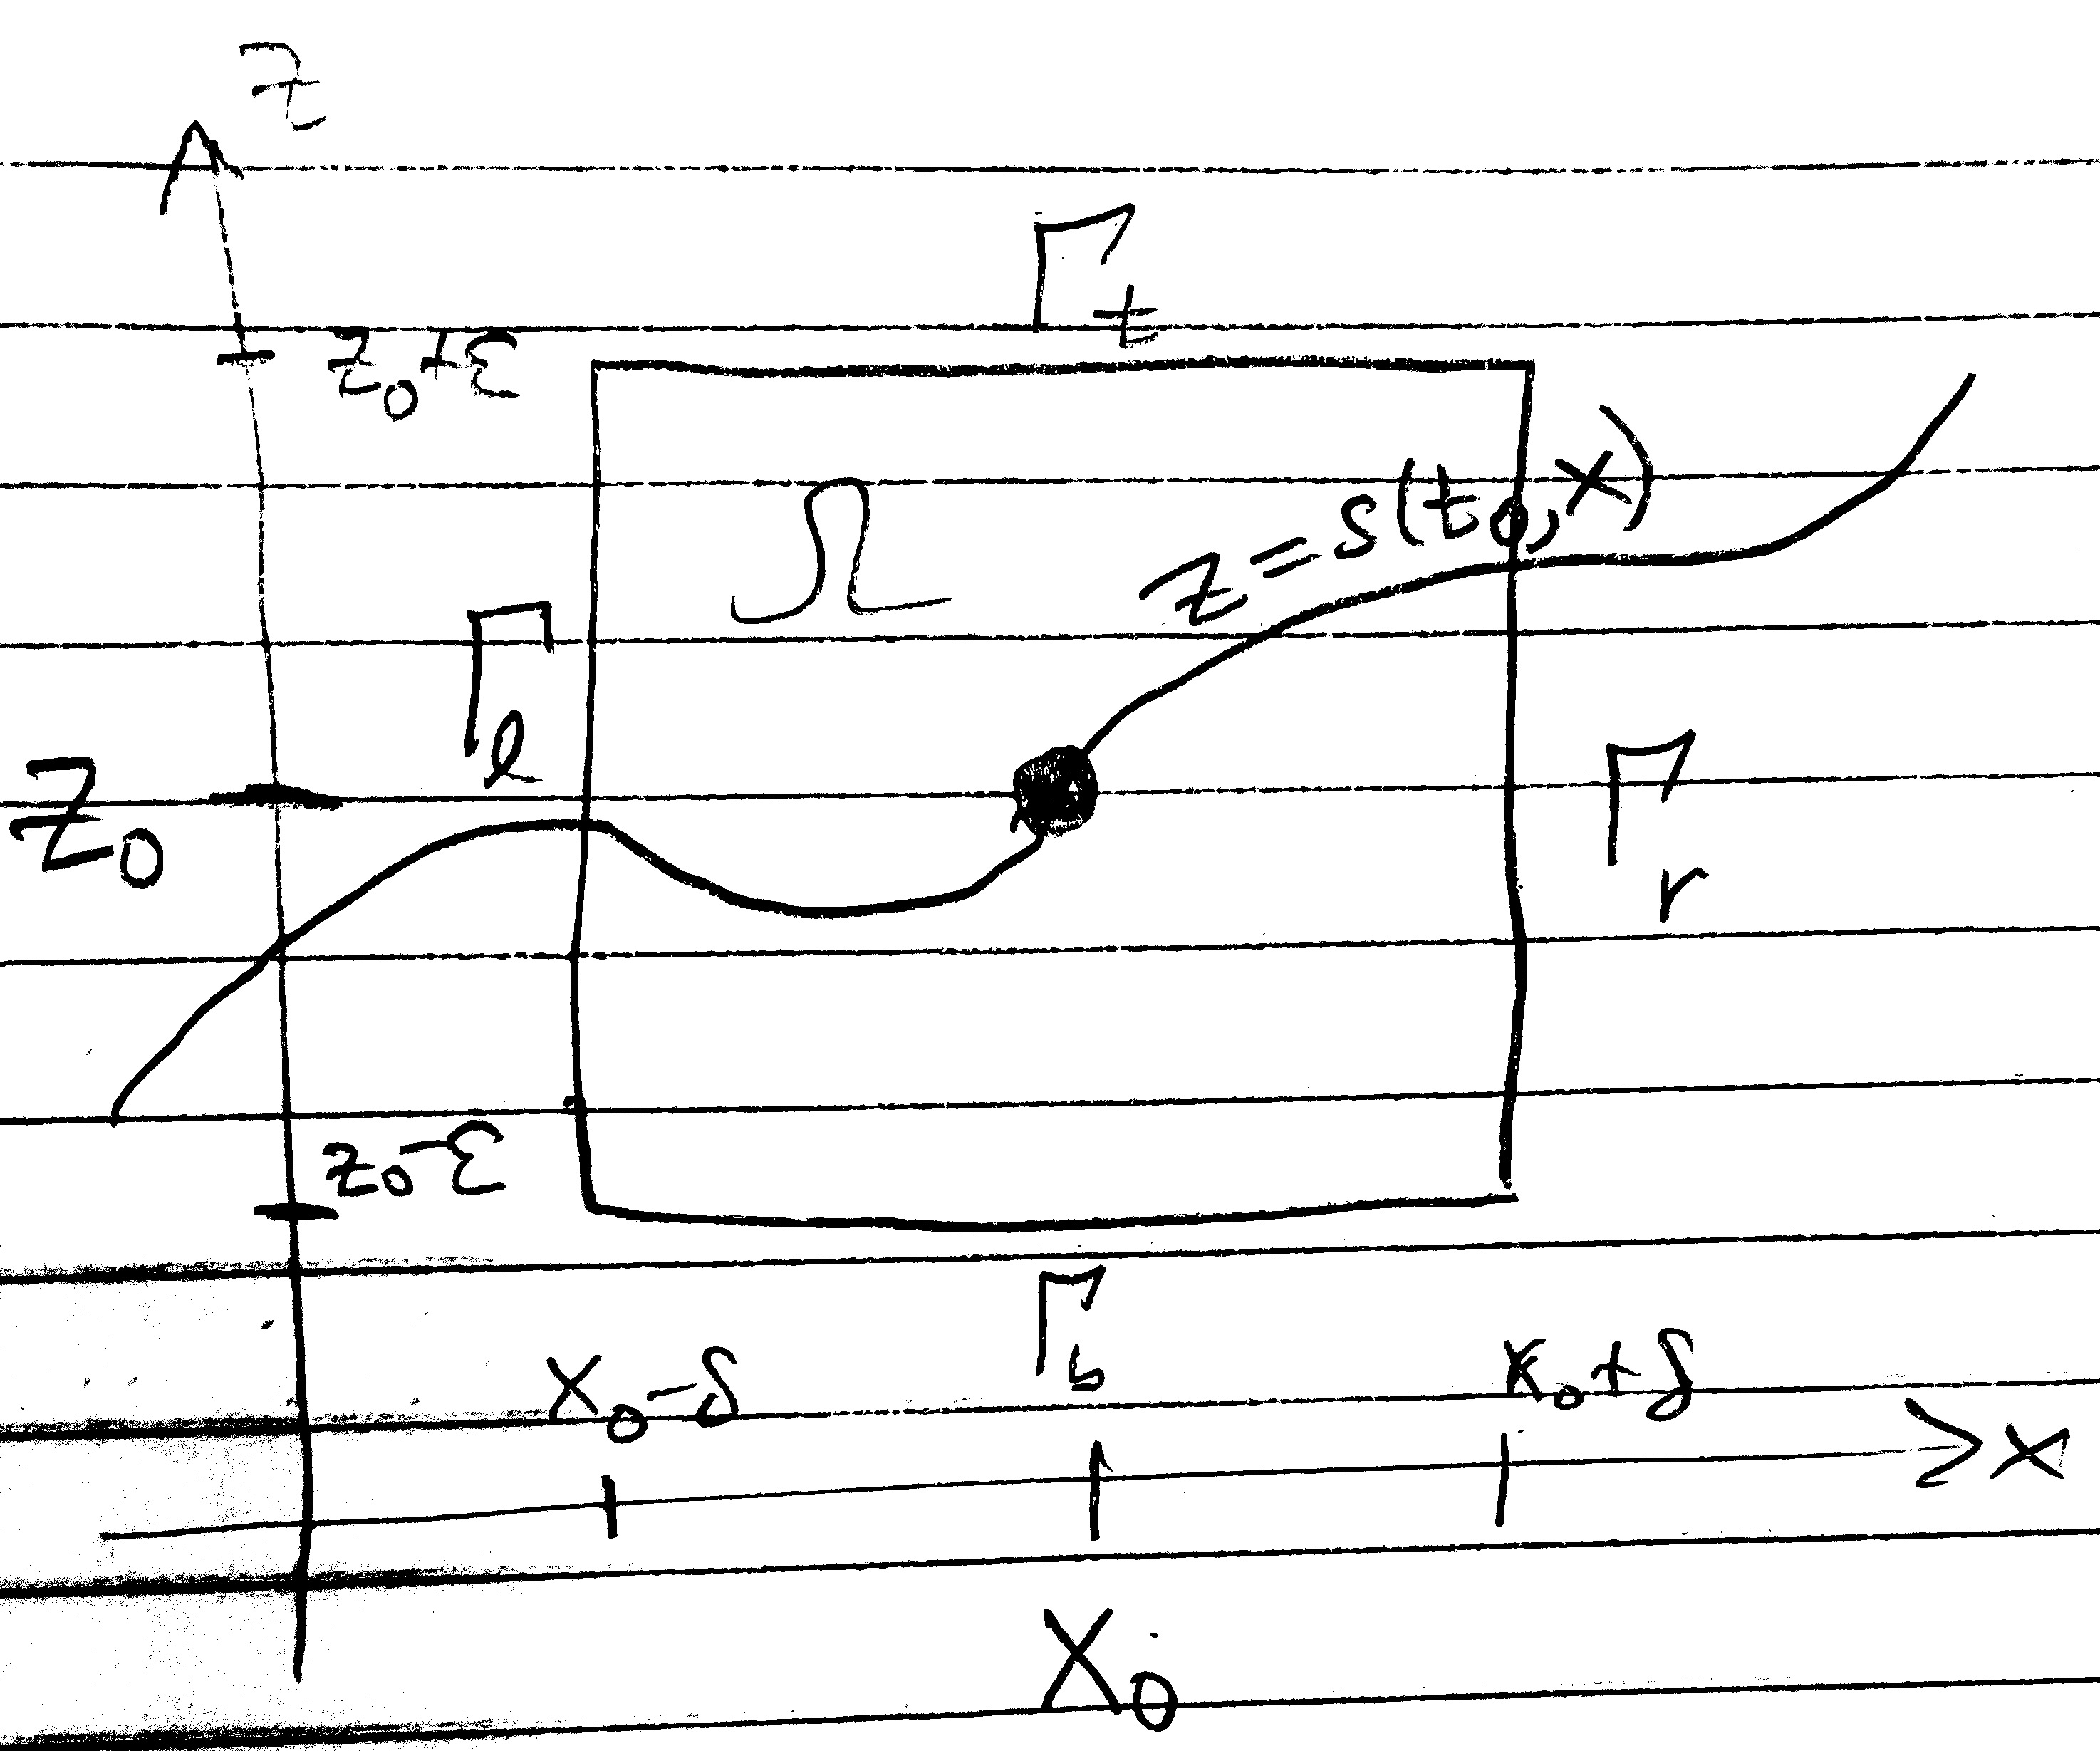
\includegraphics[width=0.3\textwidth]{skemassconservation.jpg}
\end{center}

\begin{itemize}
\item mass is conserved (no sources):
\begin{align*}
\frac{dM}{dt} &= - \int_{\partial \Omega} \bpsi \cdot \hbn\,ds \\
  &= - \underbrace{\rhoi \int_{x_0-\delta}^{x_0+\delta} a(t,x)\,dx}_{\Gamma_t} - \underbrace{\rhoi \int_{x_0-\delta}^{x_0+\delta} w(t,x,z_0-\eps)\,dx}_{\Gamma_b} \\
  &\quad - \underbrace{\rhoi \int_{z_0-\eps}^{s(t,x_0-\delta)} u(t,x_0-\delta,z)\,dz}_{\Gamma_\ell} + \underbrace{\rhoi \int_{z_0-\eps}^{s(t,x_0+\delta)} u(t,x_0+\delta,z)\,dz}_{\Gamma_r}
\end{align*}

\end{itemize}
\end{frame}

\begin{frame}{extra: SKE from mass conservation 4}

\begin{itemize}
\item time derivative:
\begin{align*}
\frac{dM}{dt} &= \lim_{\omega\to 0} \frac{M(t+\omega) - M(t)}{\omega} \\
    &= \lim_{\omega\to 0} \rhoi \int_\Omega \mathbb{1}_{\{z<s(t+\omega,x)\}} - \mathbb{1}_{\{z<s(t,x)\}}\,dx\,dz \\
    &= \rho_i \int_{x_0-\delta}^{x_0+\delta} \frac{\partial s}{\partial t}(t,x)\,dx
\end{align*}
\item Taylor expansions on $\Omega$:
\begin{align*}
a(t,x) &= a(t,x_0) + O(\delta) \\
u(t,x,z) &= u(t,x_0,z_0) + O(\delta) + O(\eps) \\
w(t,x,z) &= w(t,x_0,z_0) + O(\delta) + O(\eps) \\
\frac{\partial s}{\partial t}(t,x) &= \frac{\partial s}{\partial t}(t,x_0) + O(\delta)
\end{align*}
\end{itemize}
\end{frame}

\begin{frame}{extra: SKE from mass conservation 5}

\begin{itemize}
\item FIXME FINISH
\end{itemize}
\end{frame}

\end{document}
